\usetikzlibrary{shapes.geometric}

\begin{frame}{program crashing?}
\begin{itemize}
\item what happens on processor when program crashes?
\vspace{.5cm}
\item other program informed of crash to display message
\item use processor to run some other program
\vspace{.5cm}
\item<2-> how does hardware do this?
\item<2-> would be complicated to tell about other programs, etc.
\item<2-> instead: hardware runs designated OS routine
\end{itemize}
\end{frame}

\begin{frame}{exceptions}
\begin{itemize}
\item recall: system calls --- software asks OS for help
\vspace{.5cm}
\item also cases where hardware asks OS for help
\item different triggers than system calls
\item but \myemph<2>{same mechanism as system calls}:
    \begin{itemize}
    \item switch to kernel mode (if not already)
    \item call OS-designated function
    \end{itemize}
\end{itemize}
\end{frame}

\begin{frame}{exceptions [Venn diagram]}
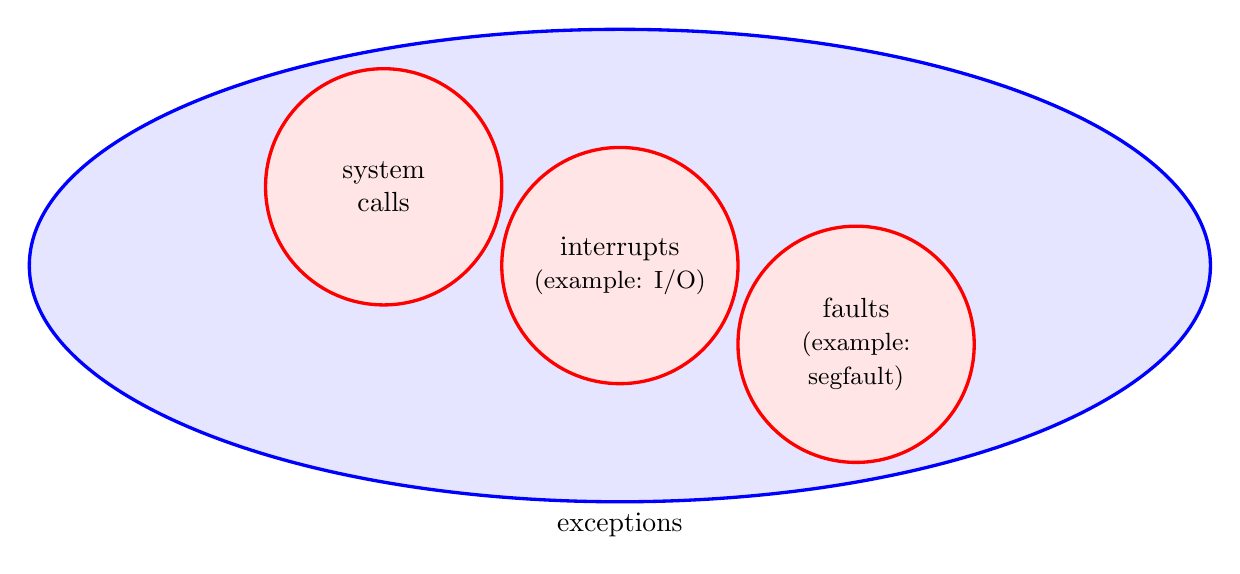
\begin{tikzpicture}
\node[very thick,draw,ellipse,blue,fill=blue!10,label={south:exceptions},minimum width=15cm,minimum height=6cm] (except) {};
\node[very thick,draw,circle,red,fill=red!10,label={[align=center]center:system\\calls},
      minimum width=3cm] (syscalls) 
    at ([xshift=-3cm,yshift=1cm]except.center){};
\node[very thick,draw,circle,red,fill=red!10,label={[align=center]center:faults\\\small (example:\\\small segfault)},
      minimum width=3cm] (fault) 
    at ([xshift=3cm,yshift=-1cm]except.center){};
\node[very thick,draw,circle,red,fill=red!10,label={[align=center]center:interrupts\\\small (example: I/O)},
      minimum width=3cm] (intr) 
    at ([xshift=0cm,yshift=0cm]except.center){};
\end{tikzpicture}
\end{frame}
